\chapter{Elements of Thin-Airfoil Theory (Linearized 2D Potential Flow)}
Assume airfoil is \emph{thin} and \emph{elongated}.
\section{Perturbation Flow- Small Perturbation Theory (Thin-Airfoil Approximation)}
\subsection{Thin airfoil assumption}
\begin{figure}[H]
\centering
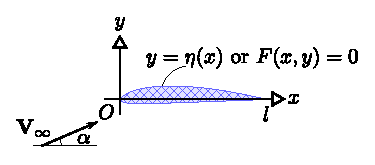
\includegraphics[scale=1.8]{figure/chapter6/6-1-1.eps}
%\caption{\label{fig:blue_rectangle} Rectangle}
\end{figure}
\begin{align*}
\alpha\ll 1, \abs{\eta(x)}\ll 1&&\text{or}&&\eta/l\ll 1,\alpha \ll 1
\end{align*}
Governing equation is
\begin{equation}
\nabla^\Phi = \frac{\partial^2\Phi}{\partial x^2} + \frac{\partial^2\Phi}{\partial y^2} = 0
\label{eq: 6-1-1}
\end{equation}
Boundary conditions are
\begin{subequations}
\begin{align}
\mathbf{v}\cdot\nabla F = 0 && \text{on $F(x,y)=0$} \label{eq: 6-1-2a}\\
\nabla\Phi\to V_\infty &&\text{at $\infty$}\label{eq: 6-1-2b}
\end{align}
\end{subequations}
\begin{align}
\text{+ KC(Kutta condition)}\colon&&\left(\nabla\Phi\right)_{\text{TE}}\text{ is finite and continuous}\label{eq: 6-1-3}
\end{align}
\begin{itemize}
\item Perturbations\\
Since $\alpha\ll 1$, $\abs{\eta}\ll 1$, can split the flow into
\begin{align*}
\mathbf{v}=\mathbf{V}_\infty + \mathbf{v'} &&\text{except }\abs{\mathbf{v'}}\ll 1
\end{align*}
where $\mathbf{v'}$ is perturbation velocity\\
i.e.
\begin{align*}
u = V_\infty\cos\alpha + u', &&v = V_\infty\sin\alpha + v'
\end{align*}
Define perturbation potential to be $\mathbf{v'}=\nabla\phi$\\
hence $\Phi = \Phi_\infty + \phi$
\[
\nabla^2\Phi = 0\Longrightarrow\nabla^2\left(\Phi_\infty+\phi\right) = 0\Longrightarrow\nabla^2\phi = 0
\]
\begin{equation}
\therefore\nabla^2\phi \equiv\frac{\partial^2\phi}{\partial x^2} + \frac{\partial^2\phi}{\partial y^2} = 0
\label{eq: 6-1-4}
\end{equation}
Boundary conditions are
\begin{subequations}
\begin{align}
\left(\mathbf{V_\infty} + \nabla\phi\right)\cdot\nabla F = 0 && \text{on $F(x,y)=0$} \label{eq: 6-1-5a}\\
\nabla^2\phi\to 0 && \text{at $\infty$}\label{eq: 6-1-5b}
\end{align}
\end{subequations}
\begin{align}
\text{+ KC(Kutta condition)}\colon&&\left(\nabla\phi\right)_{\text{TE}}\text{ is finite and continuous}\label{eq: 6-1-6}
\end{align}
\end{itemize}
\subsection{Linearized Boundary Condition}
From B.C. \eqref{eq: 6-1-5a}
\[
\left(\mathbf{V_\infty} + \nabla\phi\right)\cdot\nabla F = 0
\]
\begin{equation}
\Longrightarrow\left(V_\infty\cos\alpha+u'\right)\frac{\partial F}{\partial x} + \left(V_\infty\sin\alpha+v'\right)\frac{\partial F}{\partial y} = 0 \text{ on }F(x,y) = 0
\label{eq: 6-1-7}
\end{equation}
From now on we drop prime $'$ and the subscript represent perturbation term. 
\begin{figure}[H]
\centering
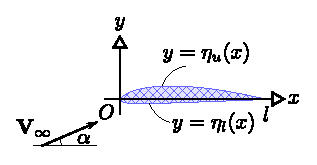
\includegraphics[scale=1.8]{figure/chapter6/6-1-2.eps}
%\caption{\label{fig:blue_rectangle} Rectangle}
\end{figure}
\begin{equation}
\eqref{eq: 6-1-7}\Longrightarrow
\frac{V_\infty\sin\alpha+ v}{V_\infty\cos\alpha+u} = \frac{-\frac{\partial F}{\partial x}}{\frac{\partial F}{\partial y}} \vc{=}{\footnotemark}{} \left(\frac{dy}{dx}\right)_{\text{body}} \equiv \frac{d\eta}{dx}
\label{eq: 6-1-9}
\end{equation}
\footnotetext{$\displaystyle dF = \frac{\partial F}{\partial x}dx + \frac{\partial F}{\partial y}dy = 0$}
(flow tangency condition on airfoil surface)
\begin{itemize}
\item Small Perturbation assumption\\
Since $\abs{\eta(x)}\ll 1$, $\alpha\ll 1$ expect velocities $u$ and $v$ be \emph{small}, i.e.
\[
\frac{u}{V_\infty},\frac{v}{V_\infty}\ll 1
\]
therefore
\begin{align*}
V_\infty\cos\alpha &\approx  V_\infty + \mathcal{O}(\alpha^2) \\
V_\infty\sin\alpha &\approx  V_\infty\alpha + \mathcal{O}(\alpha^2)
\end{align*}
\[
\eqref{eq: 6-1-9}\Longrightarrow\frac{v+V_\infty\alpha}{V_\infty}\approx\frac{d\eta}{dx}\Longrightarrow
\]
\begin{equation}
v(x,\eta)\approx V_\infty\frac{d\eta}{dx} - V_\infty\alpha\text{ on }y=\eta(x), 0\leq x\leq l
\label{eq: 6-1-10}
\end{equation}
\[
v(x,\eta) = v(x,0) + \cancel{\underbrace{\left(\frac{\partial v}{\partial y}\right)_{y=0}\eta}_{\approx \mathcal{O}(\eta^2)}}+\mathcal{O}(\eta^2)
\]
hence
\begin{align}
v(x,0)\approx V_\infty\frac{d\eta}{dx} - V_\infty\alpha, && 0\leq x\leq l
\label{eq: 6-1-11}
\end{align}
(transfer of B.C.'s)\\
for non-symmetry geometry, \eqref{eq: 6-1-11} becomes
\begin{subequations}
\begin{align}
v(x,0^+) &= V_\infty\frac{d\eta_u}{dx} - V_\infty\alpha \\
v(x,0^-) &= V_\infty\frac{d\eta_l}{dx} - V_\infty\alpha
\end{align}
for $0\leq x \leq l$
\end{subequations}
\end{itemize}
\subsection{Linearized Pressure Coefficient}
\[
p(x,y) = p_\infty + \frac{\rho}{2}V_\infty^2\left(1-\frac{V^2}{V_\infty^2}\right)
\]
where $V^2 = \left(V_\infty\cos\alpha+u\right)^2 + \left(V_\infty\sin\alpha+v\right)^2$
\[
\Longrightarrow p =p_\infty - \frac{\rho V_\infty^2}{2}\left(2\frac{u}{V_\infty}\cancelto{1}{\cos\alpha} + \frac{2v}{V_\infty}\cancelto{0}{\sin\alpha} + \cancelto{0}{\frac{u^2+v^2}{V_\infty^2}}\right)
\]
\[
\Longrightarrow p\approx p_\infty - \rho V_\infty u
\]
\[
\Longrightarrow C_p = \frac{p-p_\infty}{\frac{\rho}{2}V_\infty^2}
\]
\begin{equation}
\Longrightarrow C_p\approx-\frac{2u}{V_\infty} = -\frac{2}{V_\infty}\frac{\partial\phi}{\partial x}
\label{eq: 6-1-13}
\end{equation}
\subsection{Framework of the Thin-Airfoil Theory}
G.E.
\begin{equation}
\nabla^2\phi = \frac{\partial^2\phi}{\partial x^2} + \frac{\partial^2\phi}{\partial y^2} = 0
\label{eq: 6-1-14}
\end{equation}
B.C's
\begin{subequations}
\label{eq: 6-1-15}
\begin{align}
v(x,0^+) &= \left(\frac{\partial\phi}{\partial y}\right)_{x,0^+} = V_\infty\frac{d\eta_u}{dx} - V_\infty\alpha \label{eq: 6-1-15a}\\
v(x,0^-) &= \left(\frac{\partial\phi}{\partial y}\right)_{x,0^-} = V_\infty\frac{d\eta_l}{dx} - V_\infty\alpha \label{eq: 6-1-15b}
\end{align}
for $0\leq x \leq l$
\end{subequations}
\begin{align}
\frac{\partial\phi}{\partial x},\frac{\partial\phi}{\partial y}\to 0&&\text{as}&&x,y\to\infty
\label{eq: 6-1-16}
\end{align}
K.C.
\begin{equation}
\left(\frac{\partial\phi}{\partial x}\right)_{\text{TE}},\left(\frac{\partial\phi}{\partial y}\right)_{\text{TE}}\text{ are \emph{finite} and \emph{continuous} at TE}
\label{eq: 6-1-17}
\end{equation}
From the geometry linearlization\\
introduce a camberline function $\eta_c$
\begin{equation}
\eta_c = \frac{1}{2}\left(\eta_u+\eta_l\right)
\label{eq: 6-1-18}
\end{equation}
and thickness function $\eta_t$
\begin{equation}
\eta_t = \frac{1}{2}\left(\eta_u-\eta_l\right)
\label{eq: 6-1-19}
\end{equation}
from \eqref{eq: 6-1-18} and \eqref{eq: 6-1-19}
\begin{equation}
\begin{aligned}
\eta_u &= \eta_c + \eta_t \\
\eta_l &= \eta_c - \eta_t
\end{aligned}
\label{eq: 6-1-20}
\end{equation}
B.C. \eqref{eq: 6-1-15} becomes
\begin{subequations}
\label{eq: 6-1-21}
\begin{align}
v(x,0^+) &= \left(\frac{\partial\phi}{\partial y}\right)_{x,0^+} =  - V_\infty\alpha + V_\infty\left(\frac{d\eta_c}{dx}+\frac{d\eta_t}{dx}\right) \label{eq: 6-1-21a}\\
v(x,0^-) &= \left(\frac{\partial\phi}{\partial y}\right)_{x,0^-} =  - V_\infty\alpha + V_\infty\left(\frac{d\eta_c}{dx}-\frac{d\eta_t}{dx}\right) \label{eq: 6-1-21b}
\end{align}
for $0\leq x \leq l$
\end{subequations}
\begin{enumerate}[label = \protect\circled{\arabic*}]
\item flow past a zero-thickness flat plate at an angle-of-attack $\alpha$ 
\item flow past a zero-thickness camber at zero angle-of-attack
\item flow past a symmetric thickness airfoil at zero angle-of-attack
\end{enumerate}
\begin{figure}[H]
\centering
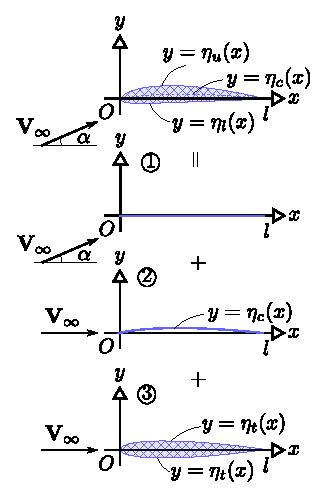
\includegraphics[scale=1.8]{figure/chapter6/6-1-3.eps}
%\caption{\label{fig:blue_rectangle} Rectangle}
\end{figure}
\section{Solutions to Elementary Thin Airfoil Problems}
\subsection{Symmetric Airfoil at Zero Angle of Attack- solution by source/sink Distribution}
\begin{itemize}
\item Governing equation
\begin{equation}
\nabla^2\phi = 0
\label{eq: 6-2-1}
\end{equation}
\begin{subequations}
\label{eq: 6-2-2}
\begin{align}
v(x,0^{\pm}) &= \left(\frac{\partial\phi}{\partial y}\right)_{x,0^{\pm}} =  \pm  V_\infty\frac{d\eta_t}{dx},0\leq x\leq l \label{eq: 6-1-2a}\\
\nabla\phi &\to 0\text{ as }x,y\to 0 \label{eq: 6-1-2b}
\end{align}
\end{subequations}
\begin{figure}[H]
\centering
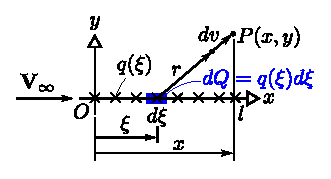
\includegraphics[scale=1.8]{figure/chapter6/6-1-4.eps}
%\caption{\label{fig:blue_rectangle} Rectangle}
\end{figure}
\begin{align}
\phi(x,y) 
&= \int d\phi = \int\frac{dQ}{2\pi}\ln r \nonumber\\
&= \frac{1}{2\pi}\int_{\xi=0}^lq(\xi)\ln\sqrt{\left(x-\xi\right)^2+y^2}d\xi\label{eq: 6-2-3}
\end{align}
and perturbation velocities $u,v$ are
\begin{subequations}
\label{eq: 6-2-4}
\begin{align}
u = \frac{\partial\phi}{\partial x} = \frac{1}{2\pi}\int_0^lq(\xi)\frac{x-\xi}{\left(x-\xi\right)^2+y^2}d\xi \label{eq: 6-2-4a}\\
v = \frac{\partial\phi}{\partial y} = \frac{1}{2\pi}\int_0^lq(\xi)\frac{y}{\left(x-\xi\right)^2+y^2}d\xi \label{eq: 6-2-4b}
\end{align}
\end{subequations}
The unknown strength $q(x)$ can be determined from the B.C. \eqref{eq: 6-1-2a}
\begin{equation}
\begin{aligned}
v(x,0^{\pm}) &= \lim_{y\to 0^\pm}\left[\frac{1}{2\pi}\int_0^lq(\xi)\frac{y}{\left(x-\xi\right)^2+y^2}d\xi\right]\\ 
&= \pm V_\infty\frac{d\eta_t}{dx}\phantom{-}(0\leq x\leq 1)
\end{aligned}
\label{eq: 6-2-5}
\end{equation}
which is \emph{Integral equation}\\
For upper surface equation \eqref{eq: 6-2-5}
\begin{align*}
v(x,0^+)
&\vc{=}{\footnotemark}{}\frac{1}{2\pi}\left\{\lim_{y\to 0^+}\left[\cancel{\int_0^{x-\delta}} + \cancel{\int_{x-\delta}^l} + \int_{x-\delta}^{x+\delta}\right]\frac{yq(\xi)}{\left(x-\xi\right)^2+y^2}d\xi\right\} \\
&=\frac{1}{2\pi}\left[\lim_{y\to 0^+}\int_{x-\delta}^{x+\delta}\frac{yq(\xi)}{\left(x-\xi\right)^2+y^2}d\xi\right]
\end{align*}
\footnotetext{for small positive $\delta$}
First, shift origin to point $x$, i.e. $\xi=x+\bar{\xi}$
\begin{align}
v(x,0^+) = \frac{1}{2\pi}\left[\lim_{y\to 0^+}\int_{\bar{\xi}= -\delta}^{\delta}\frac{yq(x+\bar{\xi})}{\bar{\xi}^2+y^2}d\bar{\xi}\right], \abs{\bar{\xi}}\ll 1
\label{eq: 6-2-6}
\end{align}
then re-scale the variable $\bar{\xi}$, i.e. let $\sigma = \bar{\xi}/y\sim\mathcal{O}(1)$
\begin{align*}
\Longrightarrow v(x,0^+) 
&= \frac{1}{2\pi}\left[\lim_{y\to 0^+}\int_{-\delta/y}^{\delta/y}\frac{q(x+y\sigma)}{\sigma^2+1}d\sigma\right] \\
&\vc{=}{\footnotemark}{y\ll 1} \frac{1}{2\pi}\lim_{y\to 0^+}\left\{\int_{-\delta/y}^{\delta/y}\frac{q(x)}{\sigma^2+1}d\sigma + y\int_{-\delta/y}^{\delta/y}\frac{q'(x)\sigma}{\sigma^2+1}d\sigma\right\} + \cdots \\
&= \frac{q(x)}{2\pi}\left\{\lim_{y\to 0^+}\int_{-\delta/y}^{\delta/y}\frac{d\sigma}{\sigma^2+1}\right\} \\
&= \frac{q(x)}{2\pi}\left\{\lim_{y\to 0^+}\left[\arctan\sigma\right]_{-\delta/y\to\infty}^{\delta/y\to -\infty}\right\} \\
&= \frac{q(x)}{2}
\end{align*}
\footnotetext{hence $q(x+y\sigma) = q(x) + q'(x)y\sigma + \mathcal{O}(y^2)$} 
Similarly, 
\[
v(x,0^-) = -\frac{q(x)}{2}
\]
i.e.
\begin{equation}
q(x) = 2v(x,0^+) = 2V_\infty\frac{d\eta_t}{dx}
\label{eq: 6-2-7}
\end{equation}
Having known the $q(x)$
\begin{align*}
\Longrightarrow u(x,y)=?, && v(x,y) = ?
\end{align*}
The pressure coefficient $C_p(x,y)$ is 
\begin{equation}
C_p(x,y) = -\frac{2u(x,y)}{V_\infty}
\label{eq: 6-2-8}
\end{equation}
Specifically, the $C_p$ on the surface of the airfoil is
\begin{subequations}
\label{eq: 6-2-9}
\begin{equation}
C_p(x,0^{\pm}) = -\frac{2u(x,0^{\pm})}{V_\infty}
\label{eq: 6-2-9a}
\end{equation}
with 
\begin{align}
u(x,0)
&= \frac{1}{2\pi}\left\{\int_{\xi=0}^lq(\xi)\frac{x-\xi}{\left(x-\xi\right)^2+y^2}d\xi\right\}_{y=0} \nonumber \\
&= \frac{1}{2\pi}\int_0^l\frac{q(\xi)}{x-\xi}d\xi = \frac{V_\infty}{\pi}\int_{\xi=0}^l\frac{d\eta_t(\xi)}{d\xi}\frac{1}{x-\xi}d\xi
\label{eq: 6-2-9b}
\end{align}
\end{subequations}
(Hilbert integral)\\
Often, transform $x,\xi$ into $\theta,\varphi$ by using
\begin{equation}
\begin{aligned}
x&=\frac{l}{2}\left(1+\cos\theta\right),  0\leq \theta\leq \pi(\text{upper}), -\pi\leq \theta\leq 0(\text{lower}) \\
\xi &= \frac{l}{2}\left(1+\cos\varphi\right),  0\leq \varphi\leq \pi(\text{upper}), -\pi\leq \varphi\leq 0(\text{lower})
\end{aligned}
\end{equation}
\begin{figure}[H]
\centering
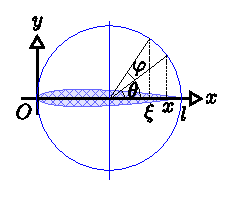
\includegraphics[scale=1.8]{figure/chapter6/6-1-5.eps}
%\caption{\label{fig:blue_rectangle} Rectangle}
\end{figure}
then \eqref{eq: 6-2-9b} becomes Poisson's Integral Formula
\begin{align}
u(\theta)
&= -\frac{1}{2\pi}\int_{\varphi = \pi}^0q(\varphi)\frac{\sin\varphi}{\cos\theta-\cos\varphi}d\varphi \nonumber\\
&= -\frac{1}{2\pi}\int_0^\pi q(\varphi)\frac{\sin\varphi}{\cos\varphi-\cos\theta}d\varphi \label{eq: 6-2-12} \\
&= -\frac{V_\infty}{\pi}\int_0^\pi\frac{d\eta_t(\varphi)}{d\xi}\frac{\sin\varphi}{\cos\varphi-\cos\theta}d\varphi \label{eq: 6-2-13}
\end{align}
(Poisson's Integral Formula)\\
notations:\\
\[
u(\theta)\equiv u(x(\theta),0^{\pm})
\]
\[
\frac{\partial\eta_+(\theta)}{dx} = \left.\frac{\partial\eta_+(x)}{dx}\right|_{x=x(\theta)}
\]
\item The pressure coefficient $C_p$ on the surface of the airfoil\\
Since $\displaystyle\frac{d\eta_t}{dx}$ (odd function in $x$ by expanding $\displaystyle\frac{d\eta_t}{dx}$ into a Fourier Sine Series), using $\displaystyle x=\frac{l}{2}\left(1+\cos\theta\right)$
\begin{equation}
\frac{d\eta_t(\theta)}{dx} = \sum_{n=1}^\infty A_n\sin n\theta\label{eq: 6-2-14}
\end{equation}
where
\begin{equation}
A_n = \frac{2}{\pi}\int_0^\pi\frac{d\eta_t(\theta)}{dx}\sin n\theta d\theta \label{eq: 6-2-15}
\end{equation}
then \eqref{eq: 6-2-13} becomes
\begin{equation}
\frac{u(\theta)}{V_\infty} = -\frac{1}{\pi}\int_0^\pi\underbrace{\left(\sum_{n=1}^\infty A_n\sin n\varphi\right)}_{\text{Given}}\underbrace{\frac{\sin\varphi}{\cos\varphi - \cos\theta}}_{\text{Kernal}}d\varphi
\label{eq: 6-2-16}
\end{equation}
Now what is $\displaystyle\int_0^\pi\frac{\sin n\varphi \sin\varphi}{\cos\varphi-\cos\theta}d\varphi=?$
first
\[
\sin n\varphi \sin\varphi = -\frac{1}{2}\left[\cos(n+1)\varphi - \cos(n+1)\varphi\right]
\]
Now define
\[
I_n(\theta) = \int_0^\pi\frac{\cos n\varphi}{\cos\varphi - \cos\theta}d\varphi
\]
\begin{enumerate}[label = \protect\circled{\arabic*}]
\item $\displaystyle I_0(\theta) = \int_0^\pi\frac{1}{\cos\varphi - \cos\theta}d\varphi = 0$
\item $\displaystyle I_1(\theta) = \int_0^\pi\frac{\cos\varphi}{\cos\varphi - \cos\theta}d\varphi = \int_0^\pi\left[1+\frac{\cos\theta}{\cos\varphi-\cos\theta}\right]d\varphi = \pi$
\item $I_2(\theta) = \cdots = 2\cos\theta I_1 = 2\pi\cos\theta$
\end{enumerate}
for general $n$
\begin{equation}
I_n = \pi\frac{\sin n\theta}{\sin\theta}
\label{eq: 6-2-19}
\end{equation}
Hence in \eqref{eq: 6-2-16}
\begin{align*}
\int_0^\pi\frac{\sin n\varphi \sin\varphi}{\cos\varphi-\cos\theta}d\varphi
&= -\frac{1}{2}\left\{\underbrace{\int_0^\pi\frac{\cos(n+1)\varphi}{\cos\varphi-\cos\theta}d\varphi}_{I_{n+1}} - \underbrace{\int_0^\pi\frac{\cos(n-1)\varphi}{\cos\varphi-\cos\theta}d\varphi}_{I_{n-1}}\right\} \\
&= -\frac{1}{2}\left[I_{n+1}-I_{n-1}\right] \\
&= -\frac{1}{2}\frac{\pi}{\sin\theta}\left[2\cos n\theta\sin\theta\right] = -\pi\cos n\theta
\end{align*}
\begin{equation}
\therefore\frac{u(\theta)}{V_\infty} = \sum_{n=1}^\infty A_n\cos n\theta
\end{equation}
where
\[
A_n = \frac{2}{\pi}\int_0^\pi\frac{d\eta_t(\theta)}{dx}\sin n\theta d\theta
\]
\begin{align}
C_p(x,0^{\pm})
&\equiv C_p(\theta)  = -\frac{2u(\theta)}{V_\infty} \nonumber\\
&= -2\sum_{n=1}^\infty A_n\cos n\theta\label{eq: 6-2-21}
\end{align}
where
\begin{align*}
0\leq\theta\leq \pi\colon && \text{upper surface}
\end{align*}
\begin{align*}
-\pi\leq\theta\leq 0\colon && \text{lower surface}
\end{align*}
\end{itemize}
\subsection{Cambered Airfoil at zero Angle-of-Attack- solution by vortices Distribution (Vortex sheet)}
\begin{figure}[H]
\centering
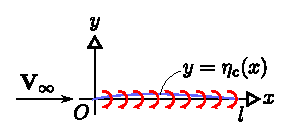
\includegraphics[scale=1.8]{figure/chapter6/6-1-6.eps}
%\caption{\label{fig:blue_rectangle} Rectangle}
\end{figure}
\begin{itemize}
\item Governing equation
\begin{equation}
\nabla^2\phi = 0
\label{eq: 6-2-25}
\end{equation}
\begin{subequations}
\label{eq: 6-2-26}
\begin{align}
v(x,0^{\pm}) &= \left(\frac{\partial\phi}{\partial y}\right)_{x,0^{\pm}} =   V_\infty\frac{d\eta_c}{dx},0\leq x\leq l \label{eq: 6-2-26a}\\
\nabla\phi &\to 0\text{ as }x,y\to 0 \label{eq: 6-2-26b}
\end{align}
\end{subequations}
K.C.
\begin{equation}
u=\frac{\partial\phi}{\partial x},v=\frac{\partial\phi}{\partial y}\text{ is finite and continuous at TE}
\label{eq: 6-2-27}
\end{equation}
\begin{figure}[H]
\centering
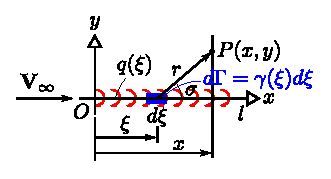
\includegraphics[scale=1.8]{figure/chapter6/6-1-7.eps}
%\caption{\label{fig:blue_rectangle} Rectangle}
\end{figure}
\begin{align}
\phi(x,y)
&= \int d\phi = \int -\frac{d\Gamma}{2\pi}\sigma = -\frac{1}{2\pi}\int_{\xi=0}^l\gamma(\xi)\sigma d\xi \nonumber \\
&= -\frac{1}{2\pi}\int_0^l\gamma(\xi)\arctan\frac{y}{x-\xi} d\xi \label{eq: 6-2-28}
\end{align}
velocities $u,v$
\begin{subequations}
\label{eq: 6-2-29}
\begin{align}
u(x,y) &= \frac{\partial\phi}{\partial x} = \frac{1}{2\pi}\int_0^l\gamma(\xi)\frac{y}{\left(x-\xi\right)^2+y^2}d\xi \label{eq: 6-2-29a}\\
v(x,y) &= \frac{\partial\phi}{\partial y} = \frac{1}{2\pi}\int_0^l\gamma(\xi)\frac{x-\xi}{\left(x-\xi\right)^2+y^2}d\xi \label{eq: 6-2-29b}
\end{align}
\end{subequations}
Now what is $\gamma(x)$ ?\\
look at $u(x,0^{\pm})$ first
\begin{equation}
\eqref{eq: 6-2-29a}\Longrightarrow
u(x,0^{\pm}) = \lim_{y\to 0^{\pm}}\left[\frac{1}{2\pi}\underbrace{\int_0^l\gamma(\xi)\frac{y}{\left(x-\xi\right)^2 + y^2}d\xi}_{\text{Improper integral}}\right]
\tag{$\ast$} \label{eq: 6-2-2-*}
\end{equation}
Again, an improper integral\\
<cf> \eqref{eq: 6-2-5},\eqref{eq: 6-2-6}$\Longrightarrow v(x,0^{+}) = q(x)/2$\\
Hence \eqref{eq: 6-2-2-*} becomes
\begin{subequations}
\label{eq: 6-2-30}
\begin{align}
u(x,0^+) &= \frac{\gamma(x)}{2} \label{eq: 6-2-30a}\\
u(x,0^-) &= -\frac{\gamma(x)}{2} \label{eq: 6-2-30b}
\end{align}
\end{subequations}
\begin{equation}
\eqref{eq: 6-2-30a},\eqref{eq: 6-2-30b}\Longrightarrow\gamma(x) = u(x,0^+)-u(x,0^-)
\label{eq: 6-2-31}
\end{equation}
From \eqref{eq: 6-2-31}, deduce
\begin{equation}
\text{KC }\Longrightarrow\gamma(x=l) = 0
\label{eq: 6-2-32}
\end{equation}
The pressure coefficient $C_p$ on the camber surface
\begin{equation}
C_p(x,0^{\pm}) = -\frac{2u(x,0^\pm)}{V_\infty} = \mp\frac{\gamma(x)}{V_\infty}
\end{equation}
where $+$ is \emph{upper surface} and $-$ is \emph{lower surface}
The lift force on the camber airfoil 
\begin{align*}
L 
&= \int_0^l\left[p(x,0^-)-p(x,0^+)\right]dx \\
&= \frac{\rho}{2}V_\infty^2\int_0^l\left[C_p(x,0^-)-C_p(x,0^+)\right]dx \\
&=\rho V_\infty\int_0^l\gamma(x)dx=\rho V_\infty\Gamma
\end{align*}
The moment (about $x=0$) on the camber airfoil is
\begin{align}
M
&= \int_0^l\left[p(x,0^+)-p(x,0^-)\right]xdx \nonumber\\
&= -\rho V_\infty\int_0^l\gamma(x)xdx\label{eq: 6-2-35}
\end{align}
lift and moment coefficients
\begin{equation}
C_L = \frac{L}{\frac{\rho}{2}V_\infty^2l} = \frac{2}{V_\infty l}\int_0^l\gamma(x)dx
\label{eq: 6-2-36}
\end{equation}
\begin{equation}
C_M = \frac{M}{\frac{\rho}{2}V_\infty^2l^2} = \frac{-2}{V_\infty l^2}\int_0^l\gamma(x)xdx
\label{eq: 6-2-37}
\end{equation}
Now $\gamma(x)$ has to be determined from B.C. \eqref{eq: 6-2-26a}
\begin{align}
v(x,0^\pm) 
&= \lim_{y\to 0^\pm} \left[-\frac{1}{2\pi}\int_0^l\gamma(\xi)\frac{x-\xi}{\left(x-\xi\right)^2+y^2}d\xi\right] = \underbrace{V_\infty\frac{d\eta_c}{dx}}_{\text{Given}}\phantom{-}(0\leq x\leq l) \nonumber\\
&= - \frac{1}{2\pi}\int_0^l\gamma(\xi)\frac{d\xi}{x-\xi} = V_\infty\frac{d\eta_c}{dx}\phantom{-}(0\leq x\leq l) \label{eq: 6-2-38}
\end{align}
(Singular integral/Hilbert integral)
\item As before; can transform $x,\xi$ into $\theta,\varphi$ by
\begin{alignat*}{4}
& x = \frac{l}{2}\left(1+\cos\theta\right)     \quad && 0\leq\theta,\varphi\leq\pi \quad && \colon \quad && \text{upper surface}\\
& \xi = \frac{l}{2}\left(1+\cos\varphi\right)     \quad && -\pi\leq\theta,\varphi\leq 0 \quad && \colon \quad && \text{lower surface}
\end{alignat*}
\begin{equation}
\eqref{eq: 6-2-38}\Longrightarrow\frac{1}{2\pi V_\infty}\int_{\varphi = 0}^\pi\underbrace{\gamma(\varphi)}_{\text{unknown}}\frac{\sin\varphi}{\cos\varphi-\cos\theta}d\varphi = \underbrace{\frac{d\eta_c(\theta)}{dx}}_{\text{Given}}
\label{eq: 6-2-41}
\end{equation}
For arbitrary shape of camber\\
Since $\displaystyle\frac{d\eta_c}{dx}$ is an even function $\Longrightarrow\displaystyle\frac{d\eta_c(\theta)}{dx}$ is an even function in $\theta$
\begin{equation}
\Longrightarrow\frac{d\eta_c(\theta)}{dx} = \frac{B_0}{2} + \sum_{n=1}^\infty B_n\cos n\theta
\label{eq: 6-2-42}
\end{equation}
where 
\begin{align*}
\underbrace{B_0 = \frac{2}{\pi}\int_0^\pi\frac{d\eta_c(\theta)}{dx}d\theta}_{\text{(average of slope)}}, &&B_n = \frac{2}{\pi}\int_0^\pi\frac{d\eta_c(\theta)}{dx}\cos n\theta d\theta
\end{align*}
Using \eqref{eq: 6-2-42}, $\eqref{eq: 6-2-41}\Longrightarrow$
\begin{equation}
\frac{1}{2\pi V_\infty}\int_0^\pi\underbrace{\gamma(\varphi)}_{\text{unknown}}\frac{\sin\varphi}{\cos\varphi-\cos\theta}d\varphi = \underbrace{\frac{B_0}{2}+\sum_{n=1}^\infty B_n\cos n\theta}_{\text{Given}}
\label{eq: 6-2-43}
\end{equation}
wish to solve $\gamma(\theta)=$?\\
Assume the solution to $\gamma(\theta)$ is
\[
\gamma(\theta) = \gamma_1(\theta) + \gamma_2(\theta) + \gamma_h(\theta)
\]
where
\begin{equation}
\frac{1}{2\pi V_\infty}\int_0^\pi\gamma_1(\varphi)\frac{\sin\varphi}{\cos\varphi - \cos\theta}d\varphi = \sum_{n=1}^\infty B_n\cos n\theta
\label{eq: 6-2-45}
\end{equation}
\begin{equation}
\frac{1}{2\pi V_\infty}\int_0^\pi\gamma_2(\varphi)\frac{\sin\varphi}{\cos\varphi - \cos\theta}d\varphi = \frac{B_0}{2}
\label{eq: 6-2-46}
\end{equation}
\begin{equation}
\frac{1}{2\pi V_\infty}\int_0^\pi\gamma_h(\varphi)\frac{\sin\varphi}{\cos\varphi - \cos\theta}d\varphi = 0
\label{eq: 6-2-47}
\end{equation}
Solution to $\gamma_1(\theta),\gamma_2(\theta),\gamma_h(\theta)$
\[
\gamma_1(\varphi) = -2V_\infty\sum_{n=1}^\infty B_n\sin n\varphi\text{ (Recall \eqref{eq: 6-2-16})}
\]
or
\begin{equation}
\gamma_1(\theta) = -2V_\infty\sum_{n=1}^\infty B_n\sin n\theta
\label{eq: 6-2-48}
\end{equation}
Recall that
\begin{align*}
I_n = \int_0^\pi\frac{\cos n\varphi}{\cos\varphi - \cos\theta}d\varphi = \pi\frac{\sin n\theta}{\sin\theta}, && n=0,1,2,\cdots
\end{align*}
which suggest
\begin{equation}
\gamma_2(\varphi) = V_\infty B_0\frac{\cos\theta}{\sin\theta}
\label{eq: 6-2-49}
\end{equation}
Also $I_0=0$, which suggest
\begin{equation}
\gamma_h(\theta) = \frac{K}{\sin\theta}
\label{eq: 6-2-50}
\end{equation}
Hence 
\begin{align}
\gamma(\theta) 
&= \gamma_1(\theta) + \gamma_2(\theta) + \gamma_h(\theta)  \nonumber\\
&= -2V_\infty\sum_{n=1}^\infty B_n\sin n\theta + \frac{V_\infty B_0}{\sin\theta}\left(\frac{\overbrace{K}^{\text{undetermined}}}{V_\infty B_0} + \cos\theta\right)
\label{eq: 6-2-51}
\end{align}
Apply K.C.
\[
\gamma(x=l) = \gamma(\theta=0)=0\Longrightarrow\left.\frac{1}{\sin\theta}\left(\frac{K}{V_\infty B_0}+\cos\theta\right)\right|_{\theta = 0} = 0
\]
\[
\Longrightarrow K = -V_\infty B_0
\]
\begin{equation}
\therefore\gamma(\theta) = -2V_\infty\left(\frac{B_0}{2}\frac{1-\cos\theta}{\sin\theta}+\sum_{n=1}^\infty B_n\sin n\theta\right)
\label{eq: 6-2-52}
\end{equation}
\item Pressure coefficient along the camber
\begin{align}
C_p(\theta)
&\equiv C_p(x(\theta),0^\pm) = -\frac{2u(x(\theta),0^\pm)}{V_\infty} \nonumber\\
&= -\frac{\gamma(\theta)}{V_\infty},0\leq \theta\leq \pi(\text{upper}), -\pi\leq \theta\leq 0(\text{lower}) \nonumber\\ 
&= B_0\frac{1-\cos\theta}{\sin\theta} + 2\sum_{n=1}^\infty B_n\sin n\theta \label{eq: 6-2-53}
\end{align}
\begin{align}
C_L
&= \frac{2}{V_\infty l}\int_{x=0}^l\gamma(x)dx, x=\frac{l}{2}\left(1+\cos\theta\right)\nonumber \\
&= \frac{1}{V_\infty}\int_{\theta=0}^\pi\gamma(\theta)\sin\theta d\theta \label{eq: 6-2-54}
\end{align}
\begin{align}
C_M 
&= -\frac{2}{V_\infty l^2}\int_{x=0}^l\gamma(x)xdx \nonumber\\ 
&= -\frac{1}{2V_\infty}\int_{\theta = 0}^\pi\gamma(\theta)\left(1+\cos\theta\right)\sin\theta d\theta
\label{eq: 6-2-55}
\end{align}
Use \eqref{eq: 6-2-52}
\begin{equation}
C_L = -\left(B_0+B_1\right)\pi
\label{eq: 6-2-56}
\end{equation}
\begin{align}
C_M 
&=B_0\frac{\pi}{4} + B_1\frac{\pi}{2} + B_2\frac{\pi}{4} \nonumber \\
&= \frac{\pi}{4}\left(B_0+B_1\right) + \frac{\pi}{4}\left(B_1+B_2\right) \nonumber \\
&= -\frac{C_L}{4} + \frac{\pi}{4}\left(B_1+B_2\right)\label{eq: 6-2-57}
\end{align}
\begin{note}
\begin{align*}
\int_0^\pi\sin n\theta \sin m\theta d\theta 
&= 0 &&\text{for }n\neq m \\
&= \frac{\pi}{2} &&\text{for }n= m
\end{align*}
\end{note}
Recall
\[
B_0 = \frac{2}{\pi}\int_0^\pi\frac{d\eta_c(\theta)}{dx}d\theta
\]
\begin{align}
B_n = \frac{2}{\pi}\int_0^\pi\frac{d\eta_c(\theta)}{dx}\cos n\theta d\theta, && \text{for }n=1,2,\cdots
\label{eq: 6-2-58}
\end{align}
\end{itemize}
\subsection{Flat-Plate Airfoil at an Angle-of-Attack $\alpha$- solution by vortices Distribution (Vortex sheet)}
\begin{itemize}
\item Governing equation
\begin{equation}
\nabla^2\phi = 0
\label{eq: 6-2-60}
\end{equation}
\begin{subequations}
\label{eq: 6-2-61}
\begin{align}
v(x,0^{\pm}) &= \left(\frac{\partial\phi}{\partial y}\right)_{x,0^{\pm}} =   -V_\infty\alpha,0\leq x\leq l \label{eq: 6-2-61a}\\
\nabla\phi &\to 0\text{ as }x,y\to 0 \label{eq: 6-2-61b}
\end{align}
\end{subequations}
K.C.
\begin{equation}
u=\frac{\partial\phi}{\partial x},v=\frac{\partial\phi}{\partial y}\text{ is finite and continuous at TE}
\label{eq: 6-2-62}
\end{equation}
\begin{figure}[H]
\centering
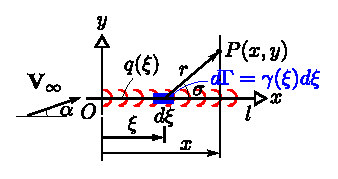
\includegraphics[scale=1.8]{figure/chapter6/6-1-8.eps}
%\caption{\label{fig:blue_rectangle} Rectangle}
\end{figure}
From previous cambered airfoil case
\begin{equation}
v(x,0^\pm) = -\frac{1}{2\pi}\int_0^l\gamma(\xi)\frac{d\xi}{x-\xi}\phantom{-}(0\leq x\leq l) 
\label{eq: 6-2-63}
\end{equation}
As before, transform $
\left\{
\begin{aligned}
&x \\
&\xi 
\end{aligned}
\right.
\Longrightarrow
\left\{
\begin{aligned}
&\theta \\
&\varphi
\end{aligned}
\right.
$
by
$
\left\{
\begin{aligned}
x&=\frac{l}{2}\left(1+\cos\theta\right) \\
\xi&=\frac{l}{2}\left(1+\cos\varphi\right)
\end{aligned}
\right.
$
\begin{equation}
\eqref{eq: 6-2-63}\Longrightarrow
v(x,0^\pm) = \frac{1}{2\pi}\int_0^l\gamma(\varphi)\frac{\sin\varphi}{\cos\varphi-\cos\theta}d\varphi = -V_\infty\alpha
\end{equation}
As before, can get $\gamma(\theta)=\gamma_2(\theta)+\gamma_h(\theta)$ <cf> \eqref{eq: 6-2-43}
\label{eq: 6-2-65}
\begin{equation}
\Longrightarrow
\gamma(\theta) = \underbrace{\frac{K}{\sin\theta}}_{\gamma_h(\theta)} - \underbrace{2V_\infty\alpha\frac{\cos\theta}{\sin\theta}}_{\gamma_2(\theta)}
\label{eq: 6-2-66}
\end{equation}
To satisfy $\gamma(\theta=0)=0\Longrightarrow K = 2V_\infty\alpha$, i.e.
\begin{equation}
\gamma(\theta) = 2V_\infty\alpha\frac{1-\cos\theta}{\sin\theta}
\label{eq: 6-2-67}
\end{equation}
\item The pressure coefficient along the flat plate 
\begin{equation}
C_p(\theta) = -\frac{\gamma(\theta)}{V_\infty} = -2\alpha\frac{1-\cos\theta}{\sin\theta}
\label{eq: 6-2-68}
\end{equation}
\begin{align*}
0\leq \theta\leq \pi\colon\text{ upper surface},&& -\pi\leq \theta\leq 0\colon\text{ lower surface}
\end{align*}
\begin{equation}
C_L = \frac{1}{V_\infty}\int_{\theta=0}^\pi\gamma(\theta)\sin\theta d\theta = 2\alpha\int_0^\pi\frac{1-\cos\theta}{\sin\theta}\sin\theta d\theta = 2\pi\alpha
\label{eq: 6-2-69}
\end{equation}
\begin{equation}
C_M = -\frac{1}{2V_\infty}\int_{\theta=0}^\pi\gamma(\theta)\left(1+\cos\theta\right)\sin\theta d\theta = -\frac{\pi}{2}\alpha = -\frac{C_L}{4}
\label{eq: 6-2-70}
\end{equation}
center of pressure
\begin{align*}
C_L = \frac{L}{\frac{\rho}{2}V_\infty^2 l}(=2\pi\alpha), &&C_M = \frac{M}{\frac{\rho}{2}V_\infty^2 l^2}(=-\frac{C_L}{4})
\end{align*}
\begin{align*}
M &= -Lx_{\text{cp}} \\
\Longrightarrow
\frac{\rho}{2}V_\infty^2l^2C_M &= \frac{\rho}{2}V_\infty^2l^2\left(-\frac{C_L}{4}\right) = -L\frac{l}{4}
\end{align*}
\begin{equation}
\therefore\boxed{x_{\text{cp}} = \frac{l}{4}}
\label{eq: 6-2-71}
\end{equation}
Aerodynamic center ($x_\text{ac}$):\\
About which the moment is independent of angle-of-attack $\alpha$. Take moment about $x=l/4$
\begin{align}
\Longrightarrow\overline{C_M} = 0&&\text{independent of }\alpha
\label{eq: 6-2-72}
\end{align}
so in the case: $x_\text{ac} = x_\text{cp} = l/4$
\end{itemize}
\subsection{Aerodynamic Characteristic of a Complete Thin Airfoil (Superposition)}
Superpose the above 3 elementary cases:\\
camber + thickness
\[
\Longrightarrow\frac{d\eta_{u,l}}{dx} = \frac{d\eta_c}{dx}\pm\frac{d\eta_t}{dx}
\]
or
\begin{equation}
\frac{d\eta(\theta)}{dx} = \frac{d\eta_c(\theta)}{dx} + \frac{d\eta_t(\theta)}{dx}, \phantom{-}\left(x=\frac{l}{2}\left(1+\cos\theta\right)\right)
\label{eq: 6-2-73}
\end{equation}
from previous results
\begin{equation}
\frac{d\eta(\theta)}{dx} = \underbrace{\frac{B_0}{2}+\sum_{n=1}^\infty B_n\cos n\theta}_{\text{camber}} + \underbrace{\sum_{n=1}^\infty A_n\sin n\theta}_{\text{thickness}}
\label{eq: 6-2-74}
\end{equation}
where
\begin{equation}
\left\{
\begin{aligned}
A_n &= \frac{2}{\pi}\int_0^\pi\frac{d\eta_t(\theta)}{dx}\sin n\theta d\theta, n=1,2,3,\cdots \\
B_0 &= \frac{2}{\pi}\int_0^\pi\frac{d\eta_c(\theta)}{dx}d\theta \\
B_n &= \frac{2}{\pi}\int_0^\pi\frac{d\eta_c(\theta)}{dx}\cos n\theta d\theta, n=1,2,3,\cdots
\end{aligned}
\right.
\label{eq: 6-2-75}
\end{equation}
Pressure distribution
\begin{align}
C_p(\theta)
&= - 2\frac{u(\theta)}{V_\infty}\nonumber \\
&= \underbrace{-2\alpha\frac{1-\cos\theta}{\sin\theta}}_{
\begin{subarray}{c}
  \text{due to flat plat}\\
  \text{at $\alpha$ angle-of-attack}
\end{subarray}
}
+
\underbrace{\left[B_0\frac{1-\cos\theta}{\sin\theta} + 2\sum_{n=1}^\infty B_n\sin n\theta\right]}_{
\begin{subarray}{c}
  \text{due to camber at}\\
  \text{zero angle-of-attack}
\end{subarray}
}
\underbrace{-2\sum_{n=1}^\infty A_n\cos n\theta}_{
\begin{subarray}{c}
  \text{due to thickness}\\
  \text{at zero angle-of-attack}
\end{subarray}
}
\label{eq: 6-2-76}
\end{align}
\begin{equation}
C_L = \underbrace{2\pi\alpha}_{
\begin{subarray}{c}
  \text{due to flat plate}\\
  \text{at $\alpha$}
\end{subarray}
}  \underbrace{-\left(B_0+B_1\right)\pi}_{
\begin{subarray}{c}
  \text{due to camber}\\
  \text{at zero}
\end{subarray}
}
\label{eq: 6-2-77}
\end{equation}
\begin{align}
C_M 
&= \underbrace{-\frac{\pi}{2}\alpha}_{
\begin{subarray}{c}
  \text{due to flat plate}\\
  \text{at $\alpha$}
\end{subarray}
} + \underbrace{\frac{\pi}{4}\left(B_0+B_1\right)+\frac{\pi}{4}\left(B_1+B_2\right)}_{
\begin{subarray}{c}
  \text{due to camber}\\
  \text{at zero}
\end{subarray}
} \nonumber \\
&= -\frac{C_L}{4}+\frac{\pi}{4}\left(B_1+B_2\right)
\label{eq: 6-2-79}
\end{align}
Take moment about $x_\text{ac} = l/4$
\begin{align}
\Longrightarrow\overline{C_M} = \frac{\pi}{4}\left(B_1+B_2\right)&&\text{independent of }\alpha
\label{eq: 6-2-80}
\end{align}
\begin{example}{a parabolic camber airfoil}
\begin{align*}
y = 4\epsilon\frac{x}{l}\left(l-x\right), &&(\epsilon\ll 1)
\end{align*}
\begin{align*}
\frac{d\eta_c}{dx}
&\equiv \frac{dy}{dx} = 4\epsilon - \frac{8\epsilon}{l}x = 4\epsilon - \frac{8\epsilon}{l}\frac{l}{2}\left(1+\cos\theta\right) \\
&=-4\epsilon\cos\theta = \frac{B_0}{2} + \sum_{n=1}^\infty B_n\cos n\theta
\end{align*}
\begin{align*}
\Longrightarrow B_0=0, && B_1 = -4\epsilon,&& B_n = 0\phantom{-}(n\geq 2)
\end{align*}
\[
C_L = 2\pi\alpha-\left(B_0+B_1\right)\pi = 2\pi\alpha + 4\epsilon\pi
\]
\[
C_M = -\frac{C_L}{4} + \frac{\pi}{4}\left(B_1+B_2\right) = -\frac{\pi\alpha}{2}-2\epsilon\pi
\]
\[
\overline{C_M} = \frac{\pi}{4}\left(B_1+B_2\right) = -\epsilon\pi\phantom{-}\text{independent of }\alpha
\]
also
\begin{align*}
\gamma(\theta)
&= 2V_\infty\alpha\frac{1-\cos\theta}{\sin\theta} - 2V_\infty\left(\frac{B_0}{2}\frac{1-\cos\theta}{\sin\theta} + \sum_{n=1}^\infty B_n\sin n\theta\right) \\
&= 2V_\infty\alpha\frac{1-\cos\theta}{\sin\theta} + 8\epsilon V_\infty\sin\theta
\end{align*}
and
\[
\Gamma = \int_{x=0}^l\gamma(x)dx = \frac{l}{2}\int_{\theta=0}^\pi\gamma(\theta)\sin\theta d\theta = \pi V_\infty l\left(\alpha +2\epsilon\right)
\]
\[
C_p(\theta) =  -2\alpha\frac{1-\cos\theta}{\sin\theta} - 8\epsilon\sin\theta
\]
\end{example}